\section{Concepts and Related Work}
\label{sec:background}

\subsection{Feature Learning}
\label{subsec:featurelearning}

Feature engineering is the practice of cleverly combining several features
to get at information that none of them could provide on their own.
For example, the $x$- and $y$-velocities of an object can be combined
to give its overall speed, or specific
patterns in a $3 \times 3$ collection of
pixels can be used to detect edges.
Feature learning, also known as \textbf{
\href{https://en.wikipedia.org/w/index.php?title=Feature_engineering&section=3}
{automated feature engineering}}, is when features are generated through
heuristics or the result of algorithms.
There are a collection of
\textbf{
\href{https://en.wikipedia.org/w/index.php?title=Feature_engineering&section=5}
{open source tools}} for this, which largely
focus on time series data sets.

Feature learning is also referred to as \textbf{
\href{https://en.wikipedia.org/wiki/Feature_learning}{representation learning}}.
\textbf{\href
{https://en.wikipedia.org/w/index.php?title=Feature_learning&section=6}
{Principal components analysis}} (PCA) is the poster child for unsupervised
representation learning. PCA resembles Ziptie in that it finds combinations
of features that tend to co-occur. PCA is focused on \textit{dimensionality
reduction} in that its goal is to reduce the total number of features used
to a small set that distills out most of the informtion in the data.

\subsection{Sparse Coding}
\label{subsec:sparsecoding}

Ziptie is an example of specific variant of feature learning called
\textbf{\href{https://en.wikipedia.org/wiki/Sparse_dictionary_learning}
{sparse coding}} or \textbf{sparse dictionary learning}, a family of methods
for learning concise ways to represent data. 

The goal of sparse coding is to represent an observation
using as few features as possible.
To do this, sparse coding methods often learn an
overcomplete dictionary of basis functions.
(Extending the analogy of a dictionary of the English language,
the basis functions are the words.
Overcomplete means that
there is more than one combination of words that express the same idea.
Overcompleteness allows for sparse representation, because you
can choose the represent the idea concisely, using the representation
with the fewest words.)

A culinary example of sparse coding is ``Moose Tracks" flavor ice cream.
It could just as accurately be described as ``vanilla with small
peanut butter cups and fudge ripples". The name ``Moose Tracks" is
superfluous; it means exactly the same thing.
Its existence shows overcompleteness in the dictionary
of ice cream flavor names. But it allows for a concise representation.

Another example of sparse coding shows up in music. As seen in
Figure~\ref{fig:chords}, combinations of several keys (features)
can be represented as chords (basis functions). There are many more
possible chords than keys. Moving to a chord representation does not
make a shorter dictionary than working with keys directly. But what
it buys us is the ability to represent a collection of several keys with
a single feature instead of having to enumerate all the keys involved. 

\begin{figure}[ht]
\vskip 0.2in
\begin{center}
\centerline{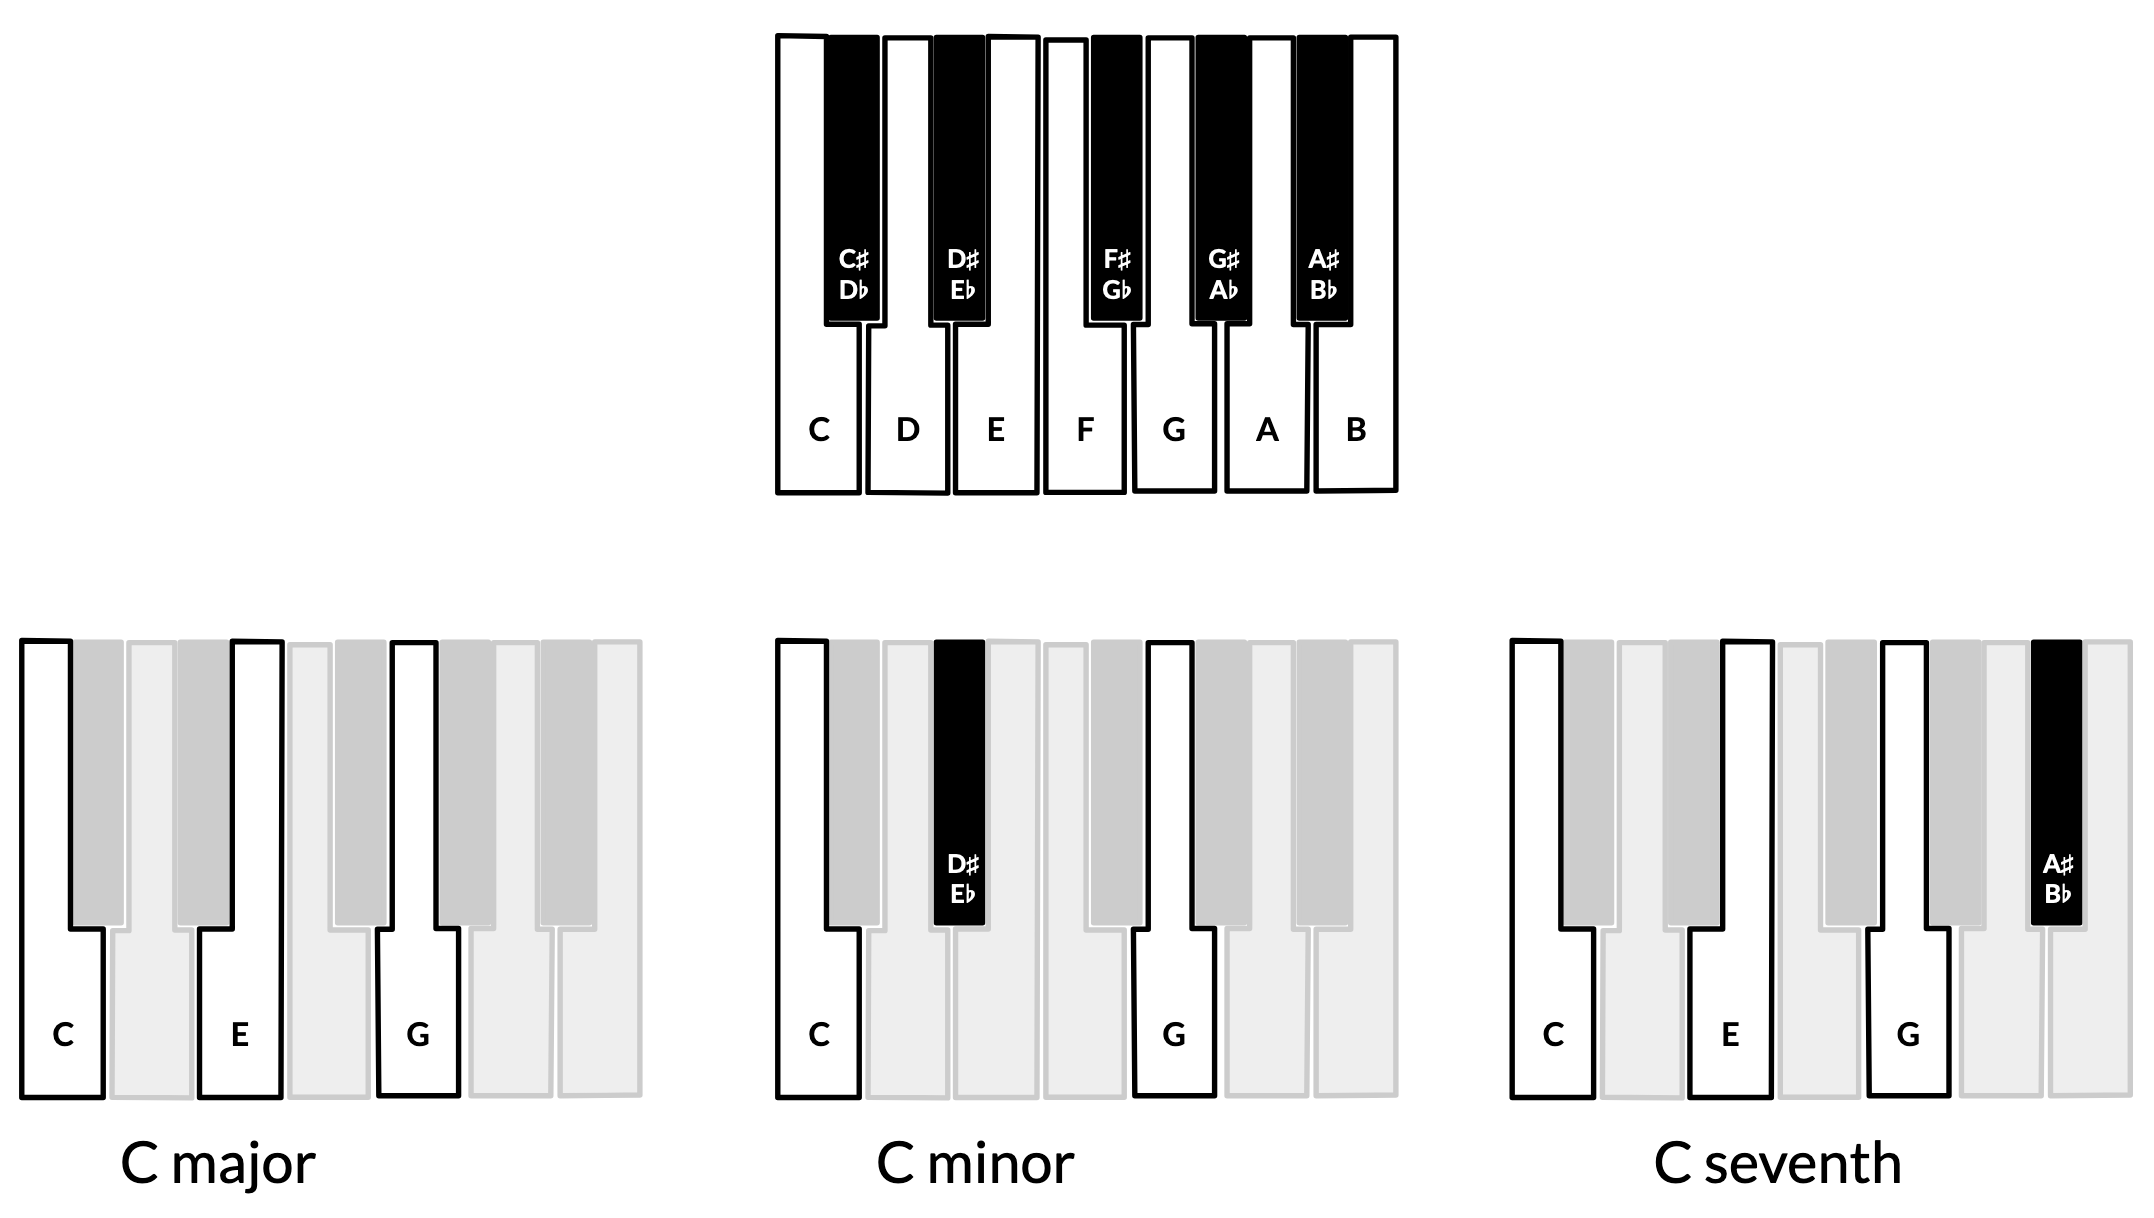
\includegraphics[width=3.25in]{images/chords.png}}
\caption{Piano chords as a sparse coding}
\label{fig:chords}
\end{center}
\vskip -0.2in
\end{figure}

\subsection{$\ell^0$ vs $\ell^1$ Norms}
\label{subsec:sparsenorms}

In its purest form, the goal of sparseness is have as many features be
zero as possible. An ideal sparse coding would be able to represent each
set of inputs with exactly one feature. The number of non-zero features
is also called the $\ell^0$ norm. An $\ell^0$ sparse coding will
do it's best to represent each input with as few features as possible.

Unfortunately, minimizing the $\ell^0$ norm for feature representation is hard.
Our regular machine learning bag of tricks for optimizing things
requires differentiability, and the $\ell^0$ norm is not differentiable. The
count of non-zero features changes sharply by one, even if the feature
value only changes from 0 to 0.001. And as that feature value changes from
0.001 to 0.1 to 10, the $\ell^0$ norm doesn't change at all.

As any experienced algorithms person will tell you, when presented
with a problem you can't solve, just ignore it and solve a different one.
In sparse coding, if ``sparse" is redefined to minimizing the $\ell^1$ norm,
instead of the $\ell^0$ norm, then it becomes differentiable, and can be
solved with familiar tools, including backpropagation and neural networks.

However, all hope is not lost. There is a whole field of optimization
for hard problems like this. (If you're trying to hire a person to do this
their past job titles will probably be Operations Research, rather than
Machine Learning.)
A \href{https://hal.science/hal-01965904/document}{2018 paper}
\footnote{Liu, Y., Canu, S., Honeine, P., Ruan., S. (2018)
K-SVD with a real L0 optimization: application
to image denoising.
Proc. 28th IEEE workshop on Machine Learning for Signal Processing (MLSP),
Aalborg, Denmark. pp.1 - 6.}
described a method for $\ell^0$ sparse coding using
one of these optimization methods (mixed integer quadratic programming).

I applaud them for tackling the honest-to-goodness sparse coding problem.
The only downside for practical use is that it is quite computationally
expensive. The authors don't say exactly how expensive, but when
they describe it as an Achilles' heel, that suggests it's not quite
ready for real time applications.

Another way to make sparse optimization easier to solve is to keep the
$\ell^0$ norm, but to relax the minimization requirement. What if we had
a method that was just pretty OK? What if it didn't necessarily
find the way to use the absolute minimum number of features each time,
but found a way to get kind of close? And what it it only took one-millionth
of the computation? This describes the path of heuristic approximation,
or to use less floofed-up language, a hack. The hack that Ziptie uses is
agglomerative clustering.

\subsection{Agglomerative Clustering}
\label{subsec:agglomeration}

This is a method of grouping observations or data points in which
the most similar are grouped together right away, then the slightly less
similar are added to those clusters. As clusters grow they can also glom on
to each other. This process of similar observations and clusters
repeatly combining to form larger clusters is
\textbf{\href{
https://en.wikipedia.org/w/index.php?title=Hierarchical_clustering&section=3
}{agglomerative clustering}}.
It's also called hierarchical clustering because when you trace the lineage
observations and mini-clusters combining, it forms a tree showing
the hierarchy of similarity between them. 

\subsection{Multi-membership Clustering}
\label{subsec:multimembership}

Ziptie is an unusual variant of agglomerative clustering where an item
can belong to multiple clusters. Here the ziptie analogy of
Figure~\ref{fig:multimember} can be helpful.
In a set of wires, imagine pulling out five of them and wrapping them
with one ziptie. Then imagine taking just two of those five, selecting another
two loose wires, and wrapping those four with another ziptie.
Two of the wires are included in both zipties. Those represent elements
with multiple cluster membership.

\begin{figure}[ht]
\vskip 0.0in
\begin{center}
\centerline{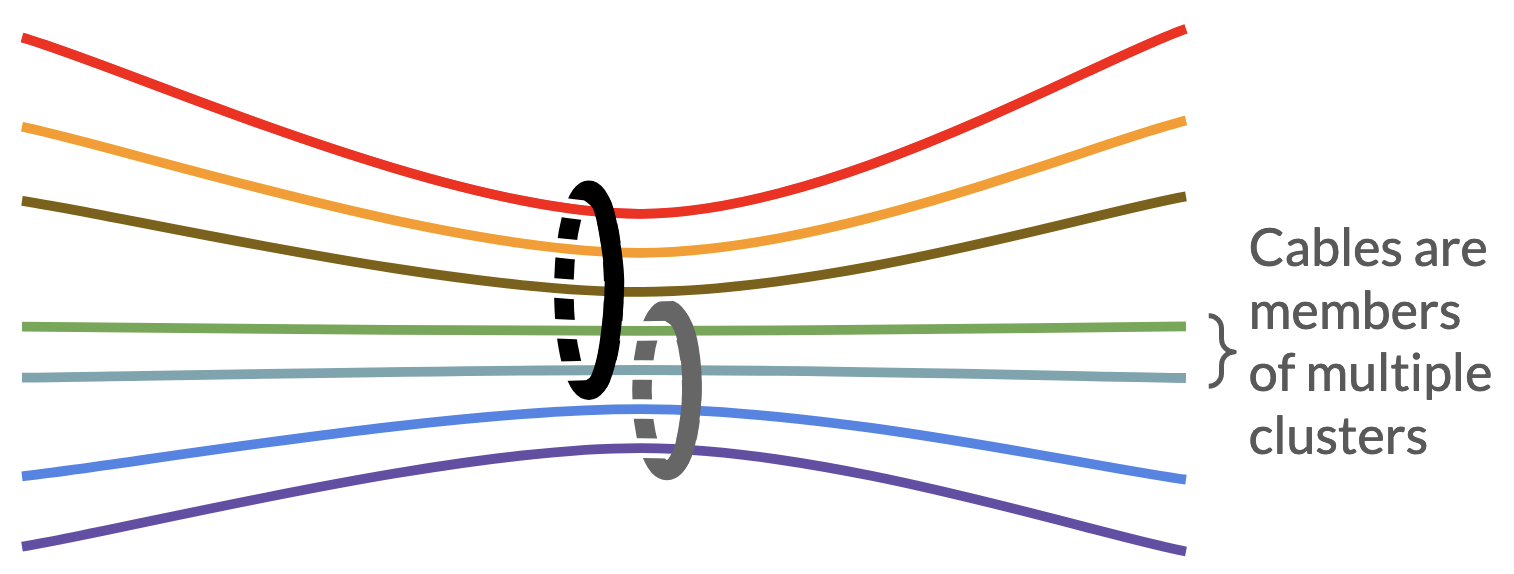
\includegraphics[width=3.0in]{images/multimember.png}}
\caption{Clustering with multiple membership.}
\label{fig:multimember}
\end{center}
\vskip -0.2in
\end{figure}

On its surface,
scikit-learn's
\href{https://scikit-learn.org/stable/auto_examples/cluster/plot_digits_agglomeration.html#sphx-glr-auto-examples-cluster-plot-digits-agglomeration-py}
{feature agglomeration}
\footnote{Pedregosa, F., Varoquaux, G., Gramfort, A., Michel, V.,
Thirion, B., Grisel, O., Blondel, M., Prettenhofer, P.,
Weiss, R., Dubourg, V., Vanderplas, J., Passos, A.,
Cournapeau, D., Brucher, M., Perrot, M., Duchesnay, E. (2011)
Scikit-learn: Machine Learning in Python. Feature agglomeration.
\textit{JMLR}, 12, 2825–2830.}
is similar to Ziptie.
It uses agglomerative clustering to group
features into larger groups of features, but it is different in
some important ways. Feature agglomeration doesn't allow for
multiple membership, and its clustering criterion is based on
correlations, rather than coactivations. More about why this matters in
Section~\ref{subsec:whycoactivation}.

Ziptie bundling process is actually more similar to
\href{https://en.wikipedia.org/wiki/Byte_pair_encoding}
{byte pair encoding} (BPE),
where frequently co-occurring characters get represented
and replaced by a unique code
of their own. The process is repeated until even long strings that
occur often are represented by a single byte.
The most important difference between Ziptie and BPE is that
BPE operates on sequences of symbols (one-hot, binary categorical variables)
and Ziptie extends the method to operate on sets of fuzzy variables.
The other minor difference is that BPE designed to work with a fixed
size batch of data. (There is some fun detail in
\href{http://www.pennelynn.com/Documents/CUJ/HTML/94HTML/19940045.HTM}
{the original writeup} from 1984.)

\subsection{Continual Learning}
\label{subsec:continual}

Continual learning is a particular case of machine learning where the
algorithm never stops evolving in response to its inputs,
\footnote{Wang, L., Zhang, X., Su, H., and Zhu, J. (2015)
A Comprehensive Survey of Continual Learning: Theory, Method and Application.
arXiv.
\href{https://arxiv.org/abs/2302.00487}{https://arxiv.org/abs/2302.00487}
}
also called incremental learning or lifelong learning.
Ziptie is a specific flavor of continual learning called
\textbf{\href{https://en.wikipedia.org/wiki/Online_machine_learning}{online learning}}
where the algorithm does a small update after every new data point is collected.
Ziptie also falls into the niche category of \textit{unsupervised}
continual learning like this
\footnote{Ashfahani, A. and Pratama, M. (2021).
Unsupervised Continual Learning in Streaming Environments. arXiv.
\href{https://arxiv.org/pdf/2109.09282.pdf}{https://arxiv.org/pdf/2109.09282.pdf}
}
and this
\footnote{Rao, D., Visin, F., Rusu, A. A., Teh, Y. W., Pascanu, R., and Hadsell, R.
(2019) Continual Unsupervised Representation Learning.
Paper presented at 33rd Conference on Neural Information Processing Systems
(NeurIPS 2019), Vancouver, Canada.
\href{https://proceedings.neurips.cc/paper_files/paper/2019/file/861578d797aeb0634f77aff3f488cca2-Paper.pdf}
{https://proceedings.neurips.cc/paper\_files/paper/2019/file/ 861578d797aeb0634f77aff3f488cca2-Paper.pdf}
}
because it isn't learning how to perform a specific task, but instead is
learning how to organize and represent its data. 


Taken all together, Ziptie sits at the intersection 
of several families of methods, as in Figure~\ref{fig:venn}.

\begin{figure}[ht]
\vskip 0.2in
\begin{center}
\centerline{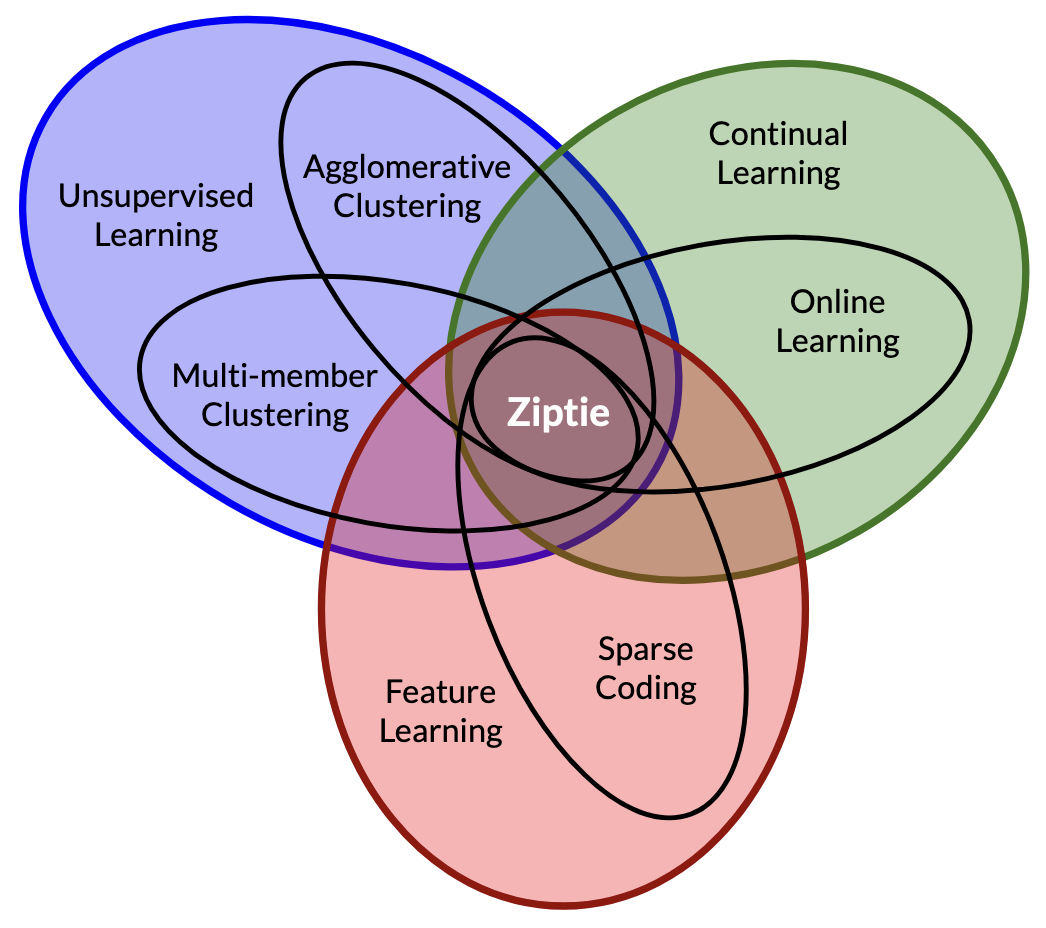
\includegraphics[width=3.0in]{images/ziptie_venn.png}}
\caption{Ziptie at the crossroads.}
\label{fig:venn}
\end{center}
\vskip -0.2in
\end{figure}

\begin{itemize}
\item{$\ell^0$ Sparse Coding}
\item{Agglomerative Clustering}
\item{Multi-member Clustering}
\item{Online Learning}
\end{itemize}
